% Haskell Symposium tutorial submission (acmsmall, lightweight double-blind).
% For publication, remove 'anonymous', 'review', and 'nonacm', and add ACM metadata.
\documentclass[acmsmall,screen,review,anonymous,nonacm]{acmart}
\usepackage{listings}
\usepackage{booktabs}
\usepackage{tabularx}
\usepackage{tikz}
\usepackage{etoolbox}
\usetikzlibrary{positioning,arrows.meta}
\settopmatter{printacmref=false}
\setcopyright{none}
\citestyle{acmauthoryear}
\lstset{language=Haskell,basicstyle=\small\ttfamily,
  columns=fullflexible,keepspaces=true,showstringspaces=false,
  commentstyle=\normalfont\ttfamily,breaklines=true,frame=single,
  xleftmargin=0.4em,xrightmargin=0.4em,aboveskip=0.7em,belowskip=0.7em}
\lstdefinestyle{output}{language={},basicstyle=\small\ttfamily,frame=none,
  backgroundcolor=\color{black!6},xleftmargin=0.4em,xrightmargin=0.4em}
% Keep commands and their results on the same page.
\BeforeBeginEnvironment{lstlisting}{\par\noindent\begin{minipage}{\linewidth}}
\AfterEndEnvironment{lstlisting}{\end{minipage}\par}
\newcommand{\code}[1]{\texttt{#1}}
\newcommand{\snippet}[1]{\par\noindent
  \begin{minipage}{\linewidth}
  \lstinputlisting{build/snippets/#1.hs}
  \end{minipage}\par}
% Listings quoted verbatim from SBV's documentation modules, which use wider lines.
\newcommand{\libsnippet}[1]{\par\noindent
  \begin{minipage}{\linewidth}
  \lstinputlisting[basicstyle=\footnotesize\ttfamily]{build/snippets/#1.hs}
  \end{minipage}\par}
\newcounter{exercise}
\newenvironment{exercise}{\refstepcounter{exercise}\par\medskip\noindent
  \textbf{Exercise~\theexercise.}\ }{\par\medskip}

\title{From Counterexamples to Inductive Proofs}
\subtitle{A Tutorial on SBV}
\author{Levent Erk\"{o}k}
\authorsaddresses{}

\begin{document}
\raggedbottom
\begin{abstract}
SBV is a Haskell library for reasoning about programs with SMT solvers. This
tutorial is a guided path through it for Haskell programmers with no prior
background in automated reasoning. We begin with one-line theorems and
counterexamples, write specifications that are independent of the code they
check, search for satisfying or optimal values, and program a live solver
session from Haskell. We then define symbolic algebraic datatypes and recursive
functions, and use induction and equational reasoning, expressed as ordinary
Haskell code, to establish properties of recursive programs. We show how proof
scripts can be reused at different element types and parameterized by operations. A
detailed proof of Kadane's maximum-segment-sum algorithm shows how to find the
right invariant, and an overview of a verified tautology checker shows how such
proofs scale. Finally, we compile a verified function to C. Along the way we
explain the boundary between Haskell evaluation and symbolic reasoning, which
often determines how a problem must be expressed. Executable listings are
extracted from checked Haskell sources; a companion validates solver results,
runs the proofs and exercise solutions, and exhaustively tests the generated
byte adder.
\end{abstract}

\keywords{Haskell, SMT, symbolic programming, theorem proving, induction, tutorial}
\maketitle

%==============================================================================
\section{Introduction}
\label{sec:introduction}

Haskell programmers already state properties of their code: QuickCheck
properties~\citep{quickcheck} can begin as ordinary functions that return \code{Bool},
and a test campaign searches for inputs that falsify them. SBV~\citep{sbv} lets
the same programmer ask a stronger question. A property over \emph{symbolic}
values is translated to logic and handed to a solver for satisfiability modulo
theories (SMT). Such a solver combines logical reasoning with theories such as
integer arithmetic and fixed-width bit-vectors. When it can settle the query,
it proves the property for every input or produces a concrete counterexample:
\begin{lstlisting}
ghci> prove $ \x -> abs (x :: SInteger) .>= 0
Q.E.D.
ghci> prove $ \x -> abs (x :: SInt8) .>= 0
Falsifiable. Counter-example:
  s0 = -128 :: Int8
\end{lstlisting}
The two properties differ only in a type. Over mathematical integers, absolute
values are nonnegative. Over signed bytes, 128 is not representable, so
\code{abs (-128)} is $-128$. The solver did not test this value by luck: it
solved a constraint whose domain contains all 256 inputs and reported a value
that fails. This does not require enumerating those inputs.

This tutorial is for Haskell programmers who want to use solvers in that way and
then go further. It assumes familiarity with type classes and monads but no
knowledge of SMT, logic, or theorem proving. Each section introduces one idea and
builds on the previous ones:
\begin{itemize}
\item Sections~\ref{sec:first}--\ref{sec:optimization} cover proofs, counterexamples,
  specifications, constraint solving, and optimization with multiple objectives.
\item Section~\ref{sec:host} explains the boundary between Haskell evaluation and
  symbolic reasoning, which governs how recursion and data structures behave.
\item Section~\ref{sec:arrays} models memory with symbolic arrays and shows why
  aliasing matters when reasoning about updates.
\item Sections~\ref{sec:queries}--\ref{sec:datatypes} program a live solver
  session and introduce symbolic algebraic datatypes.
\item Sections~\ref{sec:induction}--\ref{sec:tautology} prove properties of
  recursive functions with SBV's theorem-proving layer, TP, including polymorphic
  and higher-order proofs, and ending with a detailed
  proof of Kadane's algorithm and an overview of a verified tautology checker.
\item Section~\ref{sec:codegen} compiles a verified function to C, and
  Section~\ref{sec:hood} explains enough of the implementation to make SBV's
  behavior predictable.
\end{itemize}
Section~\ref{sec:pitfalls} collects the pitfalls in one place, and
Section~\ref{sec:related} relates SBV to other tools.

The aim is to teach a reusable method: choose a semantic domain, write a
specification, inspect counterexamples, and introduce proof structure when
automatic reasoning is insufficient. We verify functions expressed with SBV's
symbolic operations; SBV does not translate arbitrary existing Haskell source
into logic. In particular, a proof about mathematical integers or finite lists
must not be silently transferred to machine integers, partial computations, or
infinite lists.

\paragraph{Following along.}
The companion was checked with the SBV 14.10 source tree and GHC 9.14.1.
The solvers were Z3 5.3.2 and CVC5 1.4.2; the execution log records the source
revision and exact tool versions. Z3 \citep{z3} is the default solver.
The tautology-checker development also uses CVC5 \citep{cvc5}.
Install the solvers on the \code{PATH};
installing the Haskell package alone does not install them. Solver support varies
by theory, so choosing a different solver may require changing the model.

After building SBV as described in the companion's README, start GHCi from the
repository root:
\begin{lstlisting}[language={}]
cabal exec --offline -- ghci -ignore-dot-ghci -i -package sbv \
  Artifacts/Tutorial/examples/TutorialExamples.hs
\end{lstlisting}
This loads all the examples and their imports; \code{-i} ensures that GHCi uses
the built SBV package. To write a separate module, use
the following extensions and imports (some are only needed in later sections):
\snippet{extensions}
\snippet{imports}
\code{OverloadedLists} lets literals such as \code{[1,2,3]} denote symbolic lists;
\code{QuasiQuotes} enables \code{sCase}; \code{TemplateHaskell} enables datatype
generation. \code{DataKinds} and \code{TypeApplications} support named
quantifiers and explicit instantiation in proofs. \code{ScopedTypeVariables}
permits the type annotations on lambda-bound variables used below. In GHCi,
enable extensions for interactive expressions with:
\begin{lstlisting}[language={}]
:set -XOverloadedLists -XScopedTypeVariables
:set -XDataKinds -XTypeApplications
\end{lstlisting}

The companion extracts executable listings from its own source and the SBV
documentation modules. Transcripts and explicitly abbreviated listings are
presented separately. Model values and their order can vary between solver
versions; the validation checks their meaning rather than their printed form.

%==============================================================================
\section{First Proofs and Counterexamples}
\label{sec:first}

\subsection{Symbolic values and their types}

SBV's central type is \code{SBV a}, a symbolic value whose concrete counterpart
has type \code{a}. Abbreviations name the common cases: \code{SBool},
\code{SInteger} (unbounded integers), \code{SWord8} through \code{SWord64} and
\code{SInt8} through \code{SInt64} (bit-vectors with wrap-around arithmetic),
\code{SReal} (exact real numbers), \code{SFloat} and \code{SDouble} (IEEE-754),
\code{SString}, and \code{SList a}. There are also arrays, sets, tuples,
\code{Maybe}, \code{Either}, and user-defined algebraic datatypes.

These types are not interchangeable encodings of one numeric type; each is a
different mathematical problem. The introduction showed that the choice between
\code{SInteger} and \code{SInt8} changes a theorem into a false statement.
Floating point has its own surprises:
\begin{lstlisting}
ghci> prove $ \(x :: SFloat) -> x .== x
Falsifiable. Counter-example:
  s0 = NaN :: Float
\end{lstlisting}
Equality in IEEE-754 is not reflexive, and the solver knows it. Choosing a
symbolic type is choosing the semantics the solver will use, so it deserves the
same care as choosing a type for a production program.

\subsection{Operators with a dot}

Arithmetic on symbolic values uses the ordinary \code{Num} class, so \code{x + 1}
and \code{2 * y} work as expected. Comparisons cannot reuse \code{Eq} and
\code{Ord}: their methods return a Haskell \code{Bool}, which must be known when
Haskell evaluates it, while the result of comparing symbolic values may be
unknown. SBV therefore provides \code{.==}, \code{./=}, \code{.<}, \code{.<=},
\code{.>}, and \code{.>=}, which return \code{SBool}. Boolean connectives are
\code{.\&\&}, \code{.||}, \code{sNot}, and implication \code{.=>}.

For the same reason, Haskell's \code{if-then-else} cannot branch on an
\code{SBool}. The function \code{ite :: Mergeable a => SBool -> a -> a -> a}
builds a symbolic choice that the solver resolves. This distinction between
\emph{Haskell control} and \emph{symbolic control} recurs throughout the
tutorial. When all arguments are known, symbolic operations simply compute:
\code{ite ((3 :: SInteger) .> 2) 10 20 :: SInteger} evaluates to the literal \code{10} without involving a
solver.

\subsection{What \texttt{prove} does}

Calling \code{prove} on a function of symbolic arguments creates a fresh
unknown for each argument, evaluates the function to obtain a symbolic formula
$P(\vec{x})$, and asks the solver whether $\neg P(\vec{x})$ is satisfiable. If it
is not, $P$ holds for every input and SBV prints \code{Q.E.D.} If it is, the
satisfying assignment is a counterexample. A third outcome is possible: for
undecidable or very hard problems, the solver may give up or time out. SBV reports
this as an unknown result, which is neither a proof nor a refutation.

Unknowns can also be created by name inside the \code{Symbolic} monad, which
gives readable counterexamples and allows assumptions:
\begin{lstlisting}
prove $ do x <- sInteger "x"
           y <- sInteger "y"
           constrain $ x .> 0 .&& y .> 0
           pure $ x * y .> 0
\end{lstlisting}
Here \code{constrain} restricts attention to inputs that satisfy the assumption.
A contradictory assumption makes every property provable, so assumptions should
be kept as weak as the property permits. For assumptions $A$ and conclusion $P$,
\code{prove} searches for a model of $A \land \neg P$; it does not establish that
$A$ is feasible. For example,
\begin{lstlisting}
ghci> prove $ \(x :: SWord8) -> x .> 255 .=> x .== 0
Q.E.D.
ghci> sat $ \(x :: SWord8) -> x .> 255
Unsatisfiable
\end{lstlisting}
The first answer is a vacuous proof: no byte satisfies its premise. Checking the
premise with \code{sat} exposes the modeling mistake. Here and below, fresh
arguments have the default universal interpretation under \code{prove} and
existential interpretation under \code{sat}. Explicit mixed quantifiers are
possible but outside this tutorial.

Table~\ref{tab:interfaces} lists the main ways of using a symbolic model. The
rest of the tutorial visits each of them.

\begin{table}[t]
\caption{Entry points into SBV. All of them consume the same symbolic programs.}
\label{tab:interfaces}
\begin{tabularx}{\linewidth}{@{}l X X l@{}}
\toprule
Interface & You supply & Successful result & Section\\
\midrule
\code{prove} & A property & Validity or a counterexample & \ref{sec:first}--\ref{sec:specs}\\
\code{sat}, \code{allSat} & Constraints on unknowns & One or all satisfying models & \ref{sec:finding}\\
\code{optimize} & Constraints and objectives & Optimal models or objective bounds & \ref{sec:optimization}\\
\code{query} & A Haskell program driving the solver & Whatever the program computes & \ref{sec:queries}\\
TP & Lemmas, induction, calculations & Checked proofs with dependencies & \ref{sec:induction}--\ref{sec:tautology}\\
\code{compileToC} & A symbolic function & C source code & \ref{sec:codegen}\\
\bottomrule
\end{tabularx}
\smallskip
\par\small Solver calls can also be inconclusive. Enumeration can fail to
terminate, and an optimization objective need not have an attained optimum.
\end{table}

%==============================================================================
\section{Writing Specifications}
\label{sec:specs}

A proof is only as good as the property it proves. The most useful properties
compare an implementation with a specification written in a different, simpler
way. Consider addition on unsigned bytes that saturates at 255 instead of
wrapping. An implementation can avoid overflow by testing before it adds, while
the specification can use unbounded integers, where overflow cannot happen:
\snippet{saturating}
The guard \code{x .> 255 - y} cannot overflow, because \code{255 - y} is
representable for every byte \code{y}, and on the other branch \code{x + y} does
not wrap. In the specification, \code{sFromIntegral} converts each byte to an
integer \emph{before} adding. Converting the already wrapped byte sum would
repeat the implementation's arithmetic and could hide its mistakes.
\begin{lstlisting}
ghci> prove satAddSpec
Q.E.D.
\end{lstlisting}
The proof covers all 65,536 input pairs. A tempting alternative implementation
shows why the independent specification matters:
\snippet{wrongAdd}
\begin{lstlisting}[style=output]
ghci> prove $ do { x <- sWord8 "x"; y <- sWord8 "y"; pure (wrongAddSpec x y) }
Falsifiable. Counter-example:
  x = 223 :: Word8
  y = 124 :: Word8
\end{lstlisting}
The sum $223+124=347$ wraps to 91, and no byte is greater than 255, so the
saturation branch is never taken. Had the specification also used byte
arithmetic, it would have agreed with the bug. Your solver may report a different
pair; any pair whose sum exceeds 255 is a valid counterexample, and the companion
checks the reported pair with ordinary Haskell arithmetic.

\begin{exercise}
Write \code{satSub :: SWord8 -> SWord8 -> SWord8}, subtraction that saturates
at 0, together with a specification over \code{SInteger}, and prove that they
agree.
\end{exercise}

%==============================================================================
\section{Finding Values}
\label{sec:finding}

Proving a property asks whether every input satisfies it. The dual question asks
whether \emph{some} input satisfies a constraint, and which one. The function
\code{sat} returns one satisfying model, and \code{allSat} enumerates all of them.
Which bytes are unchanged by squaring?
\snippet{idempotent}
\begin{lstlisting}[style=output]
ghci> idempotentBytes
Solution #1:
  s0 = 1 :: Word8
Solution #2:
  s0 = 0 :: Word8
Found 2 different solutions.
\end{lstlisting}
The answer is a small theorem in disguise: $x(x-1)\equiv 0 \pmod{256}$, and since
$x$ and $x-1$ are coprime and $256=2^8$, one of them must be divisible by 256.
\code{allSat} repeatedly finds a model and excludes it before searching again.
The finite byte domain makes a complete enumeration possible here; on an
unbounded domain, asking for all models may never finish.

%==============================================================================
\section{Optimization}
\label{sec:optimization}

The function \code{optimize} ranks feasible solutions by named objective
\emph{measures}: \code{minimize} a cost or \code{maximize} a profit.
SBV's \code{Metric} class supports symbolic integers, reals, and bit-vectors,
among others. These objectives differ from the decreasing measures used later
to establish termination.
A workshop makes two products with profits 2 and 3, subject to two resource
limits:
\snippet{production}
Running \code{production} gives $x=4$, $y=3$, and profit 17.
Here \code{constrain} sets hard requirements. Over \code{SInteger} this is integer linear programming;
using \code{SReal} instead allows fractional production quantities. The resource
bounds ensure that the maximum is attained. In general, check for infeasibility,
unbounded objectives, and unattained bounds: maximizing a real $x$ subject to
$x<1$ has supremum 1 but no optimal model.

\paragraph{Combining measures.}
The first argument of \code{optimize} selects an \code{OptimizeStyle}:
\begin{itemize}
\item \code{Lexicographic} optimizes objectives in declaration order. Once the
  first objective is optimal, the second breaks ties, and so on. For example,
  maximize profit first, then minimize the number of units produced without
  sacrificing profit.
\item \code{Independent} uses Z3's \emph{box} mode: optimize each objective
  separately under the same constraints, returning a model for each. These
  individual optima need not be jointly attainable.
\item \code{Pareto Nothing} enumerates nondominated objective vectors: improving
  one objective requires worsening another. Their set is the \emph{Pareto front}.
  Use \code{Pareto (Just n)} to request at most $n$ such points; an infinite
  front makes unrestricted enumeration nonterminating.
\end{itemize}
For comparison, maximize nonnegative integers $x$ and $y$ with
$x+y\leq 10$. Lexicographic order $x$ then $y$ gives $(10,0)$; box gives separate
maxima $x=10$ and $y=10$; the Pareto front consists of the eleven pairs with
$x+y=10$. Box does not promise the infeasible pair $(10,10)$.

\paragraph{Bounds in an extension field.}
Extension-field results apply to both \code{SInteger} and \code{SReal}:
unbounded objectives can yield \code{oo} or \code{-oo}. Real objectives can
additionally require infinitesimals. For example, independently minimize and
maximize a positive real:
\snippet{realBounds}
Both independent results report these extension-field bounds in the tested configuration:
\begin{lstlisting}[style=output]
lower = epsilon :: Real
upper =      oo :: Real
\end{lstlisting}
Here \code{epsilon} denotes a positive infinitesimal: the infimum is 0 but is
unattained. It is not a small floating-point tolerance. The symbol \code{oo}
denotes positive infinity: the maximum is unbounded. Neither is a concrete
real assignment to \code{x}. SBV exposes such bounds through
\code{getModelObjectives} as \code{GeneralizedCV} values, using \code{ExtendedCV}
for extension-field expressions.
Changing \code{sReal} to \code{sInteger} in this example makes the minimum 1,
while the maximum remains \code{oo}.

\emph{Strict-bound pitfall.} This output is version-specific. Z3 does not
guarantee correct infinitesimal results for optimization with strict inequalities
such as \code{x .> 0}, especially when theories are mixed. Issue~5314 reports
this very minimization returning 1 instead of an infinitesimal, without an
unknown result~\citep{z3strictbounds}. Check open-bound behavior for the solver
and formulation in use; a feasible model or a successful solver status alone
does not establish optimality. Replacing $>$ by $\geq$ changes the problem.

\paragraph{Solver support and arithmetic limits.}
Z3 is currently the only optimization backend supported by SBV. SMT-LIB has
not standardized optimization commands; SBV uses Z3's extensions for objectives
and priorities~\citep{z3optimization}. Optimization is therefore less portable
across solvers than ordinary satisfiability checking.

Nonlinear arithmetic is difficult in both optimization and SMT solving generally.
Multiplying unknowns, as in \code{x * y}, leaves linear arithmetic;
\code{3 * y} remains linear.
Nonlinear integer satisfiability is undecidable, and Z3 may return unknown or
fail to finish~\citep{z3arithmetic}. Optimization must also establish that no
better solution exists. Z3 has specialized polynomial real procedures,
including improved optimization support since 5.3, but this gives no general
guarantee for nonlinear integer, mixed, or quantified problems~\citep{z3optimization}.
Prefer linear formulations where faithful to the problem, set resource limits,
and distinguish a feasible candidate from an established optimum.

%==============================================================================
\section{Haskell Structure and Symbolic Structure}
\label{sec:host}

An SBV interaction separates two kinds of work: Haskell evaluates the program
to build a symbolic formula, and the solver reasons about that formula. Query
programs can alternate between these activities. Knowing which side handles
which part of a program explains how recursion behaves.

\subsection{Haskell lists of symbolic values}

A Haskell list \code{[SInteger]} has a spine that Haskell owns and elements that
may be symbolic. Functions such as \code{sum}, \code{map}, and \code{foldr} work
on it unchanged, because they only rearrange the spine and apply \code{Num}
operations to the elements:
\snippet{hostSum}
For example, \code{prove (nonNegSum 5)} establishes the property for five
symbolic integers. Haskell
unfolds \code{sum} into \code{x1 + x2 + x3 + x4 + x5} before the solver sees
anything; the recursion has disappeared. This style is ideal for fixed-size
problems: circuits, unrolled loops, puzzles on fixed boards. The price is that
the theorem is about lists of length five, not all lists.

\subsection{Symbolic lists and recursive functions}

The type \code{SList Integer} denotes a \emph{finite} sequence whose length and
contents may both be unknown. There is no fixed length bound, but infinite lists
and partial values are outside this domain. Throughout the tutorial, a theorem
about ``every list'' means every finite list of values in the modeled element
type (Section~\ref{sec:finite-lists}). To state such a property, we need a function whose
recursion is part of the logic, not something Haskell unfolds. Writing a naive
recursive Haskell function over \code{SList} does not work: whether the list is
empty is unknown, so Haskell would unfold both branches forever.
SBV's \code{smtFunction} solves this problem. It gives the function a name, and
recursive calls become calls to that named function in the logic:
\snippet{sumL}
The \code{sCase} quasi-quoter provides pattern matching on symbolic values. The
definition reads like ordinary Haskell, but SBV translates it to a single
recursive SMT-LIB definition~\citep{smtlib}. Because \code{sumL} is a function
of symbolic values, it still computes on literals: \code{sumL [1,2,3]} evaluates
to \code{6} without a solver. When a recursive definition is registered for
symbolic reasoning, SBV checks termination; for \code{sumL}, it automatically
finds the list length as a decreasing, nonnegative measure. Termination makes
the definition admissible; it does not prove arbitrary properties of it.

Now try the obvious generalization of \code{nonNegSum}:
\snippet{sumWithoutInduction}
The property is true, but ordinary SMT reasoning about recursive definitions
does not reliably establish it. The timeout above limits each solver call to
five seconds; an unknown answer is expected with the tested configuration.
It says nothing about the truth of the property. Section~\ref{sec:induction}
supplies an induction argument that works for lists of every finite length.

The general rule is: \emph{recursion over Haskell structure happens while building
the problem; recursion through \code{smtFunction} becomes part of the problem}.
The former fixes the amount of unfolding before solving; the latter allows
statements about structures of unbounded size. Neither representation guarantees
that the resulting solver query will be easy.

%==============================================================================
\section{Arrays and Symbolic Memory}
\label{sec:arrays}

An \code{SArray Integer Integer} is a total mapping from integer addresses to
integer values. Use \code{sArray "mem"} to create an unknown array and
\code{readArray mem i} to read a symbolic address. Updates are functional:
\code{writeArray mem i v} returns an updated array, preserving \code{mem} as
the previous state.

The array theory supplies read-after-write laws: the updated address returns
the new value; all other addresses retain their values. Equality is
\emph{extensional}: equal arrays agree at every address, and
conversely~\citep{smtarrays}. Thus writes to distinct addresses commute:
\snippet{writesCommute}
\begin{lstlisting}[style=output]
ghci> prove writesCommute
Q.E.D.
\end{lstlisting}
The proof covers every initial array, both addresses, and both values. The solver
establishes equality of entire arrays directly, without traversal or induction.

Omit \code{i ./= j} and the property is false: the addresses may \emph{alias}.
For example, with $i=j=0$, $x=1$, and $y=2$, the left side stores 2 at address
0 while the right side stores 1. The last write wins, regardless of the initial
contents. The companion obtains a counterexample from the solver and checks
its updates independently using Haskell association-list lookup.

\paragraph{Bounds and the modeling domain.}
An SMT array has no built-in length, allocation status, or out-of-bounds error.
To model a buffer of length \code{n}, require \code{0 .<= i .\&\& i .< n} for a
valid access; to verify safety, prove that the program establishes this condition
before accessing the buffer. Merely assuming it would exclude invalid accesses
from the proof. \code{constArray v} initializes every address to \code{v}; a free
array has arbitrary but consistent contents.

An integer-indexed array has an infinite index domain. This does not contradict
the finite-list and recursive-datatype restriction discussed in
Section~\ref{sec:finite-lists}: an array is a total mapping, not a recursively
constructed sequence. The domain follows the index type: \code{SArray Word8 Integer}
has 256 addresses, whereas \code{SArray Integer Integer} has infinitely many.
Neither represents a partial or infinite Haskell list.

\paragraph{Bulk updates.}
The function \code{lambdaArray} describes an array by its value at each index.
The library example \code{Documentation.SBV.Examples.Misc.LambdaArray} uses it
to model range initialization: return the new value within the chosen interval
and \code{readArray mem i} outside it. This expresses both the changed region
and preservation of the remaining memory without enumerating addresses.

%==============================================================================
\section{Programming the Solver}
\label{sec:queries}

The functions \code{prove}, \code{sat}, and \code{optimize} manage solver
interactions on the caller's behalf. Many applications need a conversation: ask, inspect the
answer, and ask a refined question. SBV's \code{query} mode hands control of a
live solver session to a Haskell program. The following function finds the
smallest integer greater than 10 that leaves remainder 3 when divided by 7 and
remainder 4 when divided by 5:
\snippet{descent}
\begin{lstlisting}[style=output]
ghci> smallest
24
\end{lstlisting}
The constraints before \code{query} set up the problem as usual. Inside the
query, \code{checkSat} asks for a model, and \code{getValue} reads the value of
\code{x} in that model. That value is an ordinary \code{Integer}, so Haskell can
branch on it and use it to build the next constraint, \code{x .< literal v},
which asks for a smaller solution. When no smaller solution exists, the last
model found is the minimum. The \code{case} on the solver's answer is Haskell
control; the constraint that it adds is symbolic. Keeping the two apart is what
makes the solver usable as a component of a larger algorithm.

Three properties of this loop matter. First, successful candidates are strictly
decreasing \emph{integers} bounded below by 11. After the first candidate $v$,
there can be at most $v-11$ further decreases. Thus the loop terminates provided
each solver call returns. The existence of a minimum alone would not justify
this reasoning over reals: the candidates could decrease forever without
reaching it. Second, the solver may return the candidates in any order. Our loop
does not depend on that order; it only relies on unsatisfiability at the end.
Third, the loop handles an unknown answer separately: an inconclusive solver
response is not evidence that no smaller value exists.

Queries can do much more: \code{push} and \code{pop} add and retract temporary
assumptions, named constraints allow unsatisfiable cores to be extracted, and new
unknowns can be created in the middle of a session with \code{freshVar}. The last
point is less trivial than it looks: a new variable may have a type, such as a
user-defined datatype, that the solver has not seen yet. SBV tracks the
declarations each new term needs and sends them before the term is used, so
queries compose without regard to the order in which types are first used.

\begin{exercise}
Change \code{smallest} to find the \emph{largest} solution below 100. (The answer
is 94.)
\end{exercise}

%==============================================================================
\section{Symbolic Datatypes}
\label{sec:datatypes}

User-defined algebraic datatypes become symbolic with one line of Template
Haskell. Here is a tiny expression language and its evaluator:
\snippet{expr}
The call \code{mkSymbolic [''Expr]} generates the type \code{SExpr}, symbolic
constructors (\code{sNum}, \code{sAdd}, \code{sMul}), recognizers (\code{isNum},
\code{isAdd}, \code{isMul}), and field accessors such as \code{getMul\_1}. The
evaluator is an \code{smtFunction}, so it is a recursive definition in the
logic, and \code{sCase} matches on an expression whose constructor may be
unknown. The puzzle asks the solver to \emph{synthesize} an expression: a
multiplication whose left argument is not a number, evaluating to 42.
\begin{lstlisting}[style=output]
ghci> puzzle
Satisfiable. Model:
  s0 = Mul (Mul (Num 1) (Num (-1))) (Num (-42)) :: Expr
\end{lstlisting}
The model is an ordinary Haskell value of type \code{Expr}, which we can inspect,
print, or evaluate with a separate Haskell interpreter. The companion does exactly
that to check the answer independently of the solver. Different solver versions
may find different expressions.

The constructor test \code{isMul e} matters: an accessor such as
\code{getMul\_1 e} describes the intended field only when \code{e} has that
constructor. Also, this is synthesis from a structural constraint and one
evaluation constraint, not a proof that the expression implements a function
on every input. The search has no explicit depth bound and is not guaranteed
to terminate for arbitrary constraints.

The same datatype can be the subject of proofs: a property of \code{eval} over
all expressions concerns finite expression trees of unbounded size, and may
need induction. Infinite or partial trees are outside the model
(Section~\ref{sec:finite-lists}). Induction is the topic of the next section.

%==============================================================================
\section{Proofs by Induction}
\label{sec:induction}

SMT solvers decide many theories well, but an induction argument may be needed
to connect recursive definitions to a theorem. SBV's TP layer (in
\code{Data.SBV.TP}) lets the programmer write the
argument in Haskell and has the solver check each step. The programmer decides
\emph{what} to prove and \emph{how} to break it into steps; the solver decides
whether each step is valid.

\subsection{A first inductive proof}

We return to the property that eluded \code{prove} in Section~\ref{sec:host}:
\snippet{sumNonNeg}
The type \code{Proof (Forall "xs" [Integer] -> SBool)} records the
\emph{quantifier shape}: a property of every finite integer list \code{xs}. The actual
predicate is the first function argument to \code{induct}, stored in the proof
value; it is not encoded in this Haskell type. Two different properties can
therefore have the same \code{Proof} type. The name in \code{Forall} identifies
the quantified variable for output and instantiation. \code{TP} is the monad in
which proof scripts are built, and \code{runTP} executes a script and returns its
proof object. Typechecking the script alone does not check the theorem.

The function \code{induct} applies list induction: SBV checks the
base case (the empty list) automatically and gives the user the inductive step.
In that step, \code{ih} is the induction hypothesis, a proof of the property for
\code{xs}, and the goal is to show it for \code{x .: xs}. These cases cover
lists built by finitely many cons operations from the empty list. They do not
establish the property for infinite Haskell lists. Section~\ref{sec:finite-lists}
discusses infinite lists and explains why this restriction also applies to
recursive algebraic datatypes.

The step is a \emph{calculation}. Its first line lists the assumptions, here the
precondition for the longer list, and \code{|-} starts a chain of expressions
connected by \code{=:}. Each link must be justified by the definitions, the
assumptions, and any hints supplied with \code{??}. The chain ends with
\code{qed}. A hint written between two expressions justifies the transition
\emph{to the following expression}; \code{?? ih} is not a new assumption about
the entire theorem. In this example the expressions being equated are Boolean
formulas, and the calculation reduces the target formula to \code{sTrue}.
Running the proof shows each checked step (the final proof-object display is
omitted here):
\begin{lstlisting}[style=output]
ghci> runTP sumNonNeg
Inductive lemma: sumNonNeg
  Step: Base                  Q.E.D.
  Step: 1                     Q.E.D.
  Step: 2                     Q.E.D.
  Result:                     Q.E.D.
Functions proven terminating: sbv.foldr, sumL
\end{lstlisting}
Step~1 unfolds \code{sumL} once. Step~2 uses the hypothesis: \code{x} is
nonnegative by assumption and so is \code{sumL xs}, so the sum is too. The
\code{Result} line checks that the chain, together with the base case, establishes
the theorem as stated. The last line reports that the recursive functions used,
including the library's \code{foldr} that underlies \code{SL.all}, were checked for
termination. Section~\ref{sec:termination} explains how TP enforces this requirement.

\subsection{What the solver checks}

A calculation $e_0 = e_1 = \cdots = e_n$ under assumptions $A$, with hints
$H_i$ attached to step $i$, generates one solver query per step:
\[
  A \land H_i \land \neg(e_i = e_{i+1}) \quad\text{must be unsatisfiable.}
\]
The function definitions are available in these queries, and SBV separately
checks that the calculation establishes the stated result under its
precondition. Thus writing an unrelated true equality does not prove the
theorem. Breaking a proof into local obligations often makes it easier to solve,
although any individual obligation can still be hard. If a step fails, inspect
whether the solver found a counterexample or returned unknown. Then check the
assumptions and hint instantiations, or split the step with intermediate
expressions.

\subsection{Generalizing the statement}

Reversing a list with an accumulator is a standard optimization:
\snippet{revAcc}
We expect \code{revAcc [] xs} to equal \code{SL.reverse xs}. The direct attempt
is instructive:
\snippet{revWeak}
\begin{lstlisting}[style=output]
ghci> runTP revWeak
Inductive lemma: revWeak
  Step: Base                Q.E.D.
  Step: 1                   Q.E.D.
  Step: 2
*** Failed to prove revWeak.2.
\end{lstlisting}
Step~2 tries to use the induction hypothesis, but the hypothesis is about
\code{revAcc [] xs}, while the expression contains \code{revAcc [x] xs}. After
one step of recursion, the accumulator is no longer empty, and the hypothesis says
nothing about it. The displayed failure comes from a five-second timeout on
each solver call in the companion. It is a failure to complete this proof
attempt, not a counterexample to reversal correctness. An unrestricted solver
search might continue indefinitely.

The fix is the oldest trick in inductive proofs: prove a more general statement.
The theorem must describe \code{revAcc} for \emph{every} accumulator, so that the
hypothesis can be used at whatever accumulator the recursion produces:
\snippet{revAccCorrect}
Here \code{acc} is universally quantified, and the induction hypothesis
\code{ih} holds for all accumulators. When it is supplied as a hint, the solver
instantiates it with \code{x .: acc}. The remaining steps use ordinary laws of
\code{++} and \code{reverse}, using their sequence operations and definitions.
The original statement is the special case \code{acc = []}:
\snippet{reverseCorrect}
\code{recall} obtains the generalized proof, reusing it if it is already cached
in the current TP run. \code{proofOf} packages that proof as a dependency for
\code{lemma}, which asks the solver to establish the specialization. This
separates the reusable inductive result from the interface property callers need.

\begin{exercise}
Prove that \code{SL.length (revAcc acc xs) .== SL.length xs + SL.length acc}.
Why must the accumulator remain universally quantified in the induction
hypothesis, even when the intended caller starts with \code{[]}?
\end{exercise}

%==============================================================================
\subsection{Polymorphic scripts, monomorphic proofs}
\label{sec:polymorphic}

Reversal preserves length regardless of the element type. We can express the
proof once, using Haskell polymorphism:
\snippet{reverseLength}
The Haskell \code{forall a} makes the \emph{script} polymorphic; \code{SymVal a}
provides the symbolic representation of its elements. Before running it, we
choose a monotype. For example, in GHCi:
\begin{lstlisting}
runTP (reverseLength @Integer)
runTP (reverseLength @Word8)
\end{lstlisting}
Each invocation checks a separate theorem over that type's solver sort. The
companion runs both.

This differs from \code{Forall "xs" [a]}, which quantifies over \emph{values}
inside the theorem after \code{a} has been chosen. A successful integer instance
does not by itself certify every type instance of the script: SBV is not
quantifying over Haskell types. Polymorphism lets us reuse the argument and its
implementation, while each proof run establishes a monomorphic result. This
distinction matters especially for arithmetic laws, whose truth may change
between \code{Integer} and \code{Word8}.

%==============================================================================
\section{Higher-Order Proofs}
\label{sec:higherorder}

Many useful list laws concern an operation supplied by the caller. The
\emph{bookkeeping law}, adapted here from
\code{Documentation.SBV.Examples.TP.Lists}, says that reducing a concatenation
equals reducing each chunk and then reducing those results:
\[
 \mathit{reduce}(\mathit{concat}\ xss)
 = \mathit{reduce}(\mathit{map}\ \mathit{reduce}\ xss),
 \qquad \mathit{reduce}=\mathit{foldr}\ f\ e.
\]
Associativity of $f$ and a two-sided identity $e$ suffice. For integer addition
with identity 0, this is ``sum the elements'' versus ``sum the chunk sums.''
Commutativity is not assumed: the order of elements is preserved.
Both the outer list \code{xss} and every chunk are finite; the law makes no
claim about consuming an infinite stream of chunks.

\subsection{Proving the bookkeeping law}

We reuse a library lemma with the following import:
\snippet{listProofImports}
The proof has two dependencies: \code{foldrOverAppend}, and a helper
\code{foldBase} proved in the companion. Their conclusions are, respectively,
\[
\begin{aligned}
 \mathit{foldr}\ f\ e\ (xs \mathbin{++} ys)
   &= \mathit{foldr}\ f\ (\mathit{foldr}\ f\ e\ ys)\ xs,\\
 \mathit{foldr}\ f\ y\ xs &= f\ (\mathit{foldr}\ f\ e\ xs)\ y.
\end{aligned}
\]
The first needs no assumptions on $f$. The second requires associativity and
the left-identity law. Its empty-list case uses
$f\ e\ y=y$; its inductive step uses associativity to move $y$ past the head.
These lemmas expose exactly the two transformations the main induction needs:
\snippet{bookKeeping}
\code{quantifiedBool} packages a quantified property as an \code{SBool}, so the
algebraic laws can appear as assumptions in the calculation and as the premise
of the theorem. They are not unconditionally added as user axioms. Induction
is over the outer list of chunks: unfold \code{concat}, move the fold across
append, use the induction hypothesis on the remaining chunks, then use
\code{foldBase} to combine their result with that of the first chunk.

The left-identity assumption has a concrete purpose. Take $f\ x\ y=x$ and
$e=0$. This operation is associative and has right identity 0, but for
\code{xss = [[],[1]]}, the two sides of the bookkeeping law are 1 and 0.
The empty first chunk contributes an identity that must work on the left.
The companion checks this counterexample as well as the proof.

\subsection{An arbitrary operation at a fixed type}

The parameters \code{e} and \code{f} are Haskell arguments to the proof script.
To prove the law without choosing an implementation of the operation, give
them fresh uninterpreted names:
\snippet{bookKeepingRun}
With \code{uninterpret}, a logical constant or function has no defining equations.
Here \code{combine} is a total function on integers; the proof must
work for every interpretation satisfying the stated algebraic laws. The solver
does not enumerate implementations of \code{combine}. SBV specializes its list
operations to this logical operation and reasons about the resulting
definitions. The higher-order Haskell interface thus supports a proof about an
arbitrary operation at a fixed type. We do not pass a Haskell function as an
ordinary \code{Forall} argument of the theorem.

Passing \code{0} and \code{(+)} instead gives a concrete instance. The companion
also checks that instance and derives the unconditional sum-of-chunk-sums law.
An uninterpreted operation represents a total mathematical function; it does
not model divergence or exceptions in a Haskell callback.

\subsection{Closures and higher-order functions}
\label{sec:closures}

A callback may also depend on data from its surrounding scope. Ordinary Haskell
allows \code{map (+k) xs}, but \code{SL.map (+k) xs} cannot capture a symbolic
unknown \code{k} from the enclosing solver context in the callback's definition.
Use an explicit \code{Closure} to pass that environment:
\snippet{closure}
The environment \code{k} is symbolic data; \code{closureFun} is closed with
respect to it because it receives \code{env} as an argument. SBV carries the
environment through the generated recursive definition alongside the list.
The companion proves that \code{shiftEach} preserves length for every offset
and every finite integer list.

This restriction concerns captured symbolic unknowns, not literals or globally
named logical symbols. For example, \code{SL.map (+1)} needs no explicit closure.
The uninterpreted names above also need no captured environment: they belong
to the logical signature. Higher-order arguments describe which operation to use; a
\code{Closure} additionally supplies the changing symbolic data it needs.

%==============================================================================
\section{Case Study: Kadane's Algorithm}
\label{sec:kadane}

The maximum segment sum problem asks for the largest sum of a contiguous segment
of a list, where the empty segment has sum 0. For
\code{[1, -2, 3, 4, -1, 2]}, the answer is 8, from \code{[3, 4, -1, 2]}.
Kadane's algorithm~\citep{bentley} solves it in a single left-to-right pass.
Its correctness is not obvious, which makes it a good example of finding and
proving an invariant.

\subsection{Specification}

We specify the problem by its most direct recursive reading:
\snippet{mss}
\code{mssBegin xs} is the best sum of a segment that starts at the beginning of
\code{xs}: either the empty segment (0), just the head, or the head followed by
the best segment starting at the tail. \code{mss xs} is the best of
\code{mssBegin xs} and the best segment of the tail: a segment either starts at
the head or lies entirely in the tail. With unit-cost arithmetic and without
memoizing calls across suffixes, these recurrences take quadratic time. Since they are
symbolic functions, they also run on literal lists, which is a convenient way to
test a specification before reasoning about it:
\code{mss [1, -2, 3, 4, -1, 2]} evaluates to \code{8}.

To check that the recurrence matches the intended problem, we can independently
enumerate segments with ordinary Haskell's \code{Data.List.inits} and
\code{Data.List.tails}:
\snippet{segmentOracle}
Every segment is a prefix of a suffix, and the empty segment ensures the
maximum is defined even for \code{[]}. The companion compares both \code{mss}
and \code{kadane} against this oracle on all 3,906 lists of length at most five
over $\{-2,-1,0,1,2\}$, plus the examples above. These tests check the connection
to the intended specification; the theorem below establishes equivalence for
every finite integer list.

\subsection{Implementation}

Kadane's algorithm maintains two accumulators while it scans the list:
\code{meh}, the maximum sum of a segment ending at the current position, and
\code{msf}, the maximum found so far:
\snippet{kadane}
At each element \code{h}, the best segment ending here either extends the best
segment ending at the previous position or is empty, so the new \code{meh} is
\code{0 `smax` (h + meh)}. The best so far is updated if that value is larger.
The allowance of an empty segment matters: an all-negative input returns 0.
An API that requires a nonempty segment would need a different specification
and initialization.

\subsection{Finding the invariant}

As with reversal, the theorem we want, \code{kadane xs .== mss xs}, concerns the
initial accumulators \code{0} and \code{0}. An inductive proof will reach
\code{kadaneHelper} with other accumulator values, so we must describe what
\code{kadaneHelper xs meh msf} computes for \emph{any} sensible \code{meh} and
\code{msf}.

Think of the list as split into a prefix that has been processed and a suffix
\code{xs} that has not. The best segment of the whole list lies in one of three
places:
\begin{enumerate}
\item entirely within the prefix: its sum is \code{msf};
\item entirely within the suffix: its sum is \code{mss xs};
\item across the boundary: it is a segment ending at the boundary, whose best sum
  is \code{meh}, followed by a segment starting at the boundary, whose best sum is
  \code{mssBegin xs}.
\end{enumerate}
For example, split \code{[1,-2,3,4,-1,2]} after the 4. The processed prefix has
$\mathit{meh}=7$ and $\mathit{msf}=7$, while the suffix has
$\mathit{mss}=2$ and $\mathit{mssBegin}=1$. The three candidates are 7, 2, and
$7+1=8$; the best segment crosses the boundary.
So the invariant is
\[
  \mathit{kadaneHelper}(xs, \mathit{meh}, \mathit{msf})
  = \max\bigl(\mathit{msf},\ \mathit{mss}(xs),\ \mathit{meh} + \mathit{mssBegin}(xs)\bigr),
\]
under the preconditions that make the accumulators meaningful:
$\mathit{meh} \geq 0$ (the empty segment is always available) and
$\mathit{msf} \geq \mathit{meh}$ (the best segment so far is at least as good as
the best one ending here). Without the preconditions the statement is false: for
an empty \code{xs}, the right side would include $\mathit{meh}$ even when it
exceeds $\mathit{msf}$.

\subsection{The proof}

Once the invariant is written down, the proof is short:
\snippet{kadaneCorrect}
The inductive step unfolds \code{kadaneHelper} once and applies the hypothesis
at the new accumulators. Here the hint is more specific than in the earlier
proofs: \code{ih `at` (Inst @"meh" meh', Inst @"msf" msf')} instantiates the
quantified accumulators explicitly. The solver could search for the
instantiation, but stating it makes the step easier and documents the argument.
The remaining equality between the instantiated hypothesis and the invariant
for \code{a .: as} is arithmetic over \code{smax}, which the solver checks
without further help, using the definitions of \code{mss} and \code{mssBegin}.
The preconditions are needed to instantiate the hypothesis: the new accumulators
satisfy them because \code{meh'} is a maximum with 0 and \code{msf'} is a
maximum with \code{meh'}.

The main theorem then follows by a calculation without induction. With both
accumulators 0, the invariant gives
$\max(0, \mathit{mss}(xs), \mathit{mssBegin}(xs))$, and the solver discharges the
last two steps: \code{mss} is nonnegative and at least \code{mssBegin} by its
definition.
\begin{lstlisting}[style=output]
ghci> runTP kadaneCorrect
Inductive lemma: kadaneInvariant
  Step: Base                        Q.E.D.
  Step: 1                           Q.E.D.
  Step: 2                           Q.E.D.
  Result:                           Q.E.D.
Lemma: kadaneCorrect
  Step: 1                           Q.E.D.
  Step: 2                           Q.E.D.
  Step: 3                           Q.E.D.
  Step: 4                           Q.E.D.
  Result:                           Q.E.D.
Functions proven terminating: kadaneHelper, mss, mssBegin
\end{lstlisting}
The proof establishes equality of the two functions. The linear traversal of
\code{kadaneHelper} follows separately from its one recursive call on the tail
per element; the theorem does not establish a running-time or space bound for
Haskell evaluation, and integer arithmetic itself is not constant-cost in general.

\subsection{Lessons}

The effort in this proof went into one place: the invariant. Once we had
explained \emph{why} the algorithm works, as the three-way case analysis on where
the best segment lies, the mechanical checking was immediate. This division of
labor is typical of TP. The solver handles unfolding definitions, arithmetic,
and case analysis on \code{smax}; the human supplies generalizations and
intermediate statements. When a proof gets stuck, the useful question is
rarely ``which tactic is missing?'' and usually ``what is the statement that
explains this step?''

%==============================================================================
\section{Case Study Overview: A Verified Tautology Checker}
\label{sec:tautology}

Larger developments are built from the same ingredients. SBV's documentation
includes a verified tautology checker for propositional formulas in
if-then-else form, after a classic development by \citet{boyermoore} that was
later formalized in Imandra~\citep{imandraTautology}. We sketch its structure
rather than its proofs; the full development is in the module
\code{Documentation.\allowbreak SBV.\allowbreak Examples.\allowbreak TP.\allowbreak TautologyChecker}. The listings in this
section are quoted from that module.

\paragraph{Formulas and normalization.}
A formula is a constant, a variable, or a conditional:
\libsnippet{tautFormula}
The checker first normalizes a formula so that no conditional appears in the
condition position of another conditional, by repeatedly rewriting
\code{If (If p q r) l r'} to \code{If p (If q l r') (If r l r')}. Abbreviated
slightly, the definition is:
\begin{lstlisting}
normalize :: SFormula -> SFormula
normalize = smtFunctionWithMeasure "normalize"
    ( \f -> tuple (ifComplexity f, ifDepth f)
    , [measureLemma ifDepthNonNeg, measureLemma ifComplexityPos, ...] )
  $ \f -> [sCase| f of
             If (If p q r) l r' -> normalize (sIf p (sIf q l r') (sIf r l r'))
             If c l r           -> sIf c (normalize l) (normalize r)
             _                  -> f
          |]
\end{lstlisting}
This function is the first new ingredient. Its termination is not structural:
the rewrite in the first branch produces a \emph{larger} formula. Instead of
letting SBV guess a measure, the definition supplies one through
\code{smtFunctionWithMeasure}: a pair
ordered lexicographically. To see why this works, write $C$ for
\code{ifComplexity} and $D$ for \code{ifDepth}. On constants and variables,
$C=1$ and $D=0$; on conditionals,
\[
 C(\mathit{If}\ c\ l\ r)=C(c)\bigl(C(l)+C(r)\bigr),
 \qquad D(\mathit{If}\ c\ l\ r)=1+D(c).
\]
The distributive rewrite preserves $C$ exactly and reduces $D$ by one.
Recursing into either branch of an ordinary conditional strictly reduces $C$,
because every complexity is positive. Thus each recursive call decreases the
pair, even though tree size may increase. Each \code{measureLemma} supplies a
proved fact needed for these checks, such as positivity of $C$. Termination and
truth preservation remain separate obligations.

\paragraph{Checking.}
On a normalized formula, the checker walks down the conditionals, recording an
assumed value for each variable the first time it is tested. When it meets a
variable that was already assigned, it follows the corresponding branch;
otherwise it checks both branches, once under each assumption. The function
\code{isTautology f} normalizes \code{f} and runs this walk with no assumptions.

\paragraph{The theorems.}
Soundness says that a formula accepted by the checker evaluates to true under
every assignment:
\libsnippet{tautSoundness}
Completeness says that if the checker rejects a formula, a companion function
\code{falsify} produces an assignment under which the formula is false:
\libsnippet{tautCompleteness}
Both top-level proofs are short because the work is in their lemmas. The
development contains 21 TP lemmas. Several prove properties of variable lookup
when assignments are extended; others establish that normalization produces a
normal formula and preserves meaning. The central inductive lemmas, such as
\code{tautologyImpliesEval}, use \emph{strong induction} via \code{sInduct}:
the hypothesis is available for every formula with a smaller measure, not only
for immediate subformulas, which matches the shape of the recursion in
\code{isTautology'}. The lemmas use \code{recall} to reuse previously proved
results and, in a few places, select CVC5 instead of Z3 for steps where it
performs better. The companion checks both top-level theorems, including their
dependencies; its log records timings as diagnostics rather than benchmarks.

\paragraph{What to take away.}
The development reuses every technique from the earlier sections at larger
scale. Generalization appears again: the central lemma \code{tautologyImpliesEval} is
stated for arbitrary variable assignments, not only for the empty list of
assumptions with which \code{isTautology} starts. New
techniques are explicit termination measures and strong induction. The structure
of the proof follows the structure of the program: one group of lemmas per
auxiliary function, and top-level theorems assembled from them by short
calculations. SBV's documentation contains about forty further TP developments,
including sorting algorithms, a semantics-preserving constant folder, and a
compiler from expressions to a stack machine.

%==============================================================================
\section{From Verified Code to C}
\label{sec:codegen}

The symbolic programs we have written can also be compiled. SBV translates a
symbolic function to C code that runs without a solver. For the saturating adder
of Section~\ref{sec:specs}:
\snippet{codegen}
This produces \code{sat\_add.c} and a matching header. Because the C code is
generated from the same \code{satAdd} that we proved correct, there is no manual
rewrite in which the two could drift apart. For this adder, the generated header
maps \code{SWord8} to \code{uint8\_t}, and the arithmetic helpers implement
8-bit modular addition and subtraction using unsigned intermediates and masks.

Code generation is not a verified compiler, and it is worth being precise about
what is known. The proof establishes a property of the \emph{symbolic} function.
The C program is a separate artifact, produced by a translation that must
implement each operation faithfully. For a function with a small input domain we
can check the compiled artifact exhaustively: the companion compiles the generated adder with
undefined-behavior sanitization and compares it on all 65,536 inputs with an
independent oracle written directly in C. The proof and the exhaustive test
make different claims, about the model and about this compiled code. Exhaustive
agreement covers the tested executable and input domain; it is not a proof of
the backend for all programs, compilers, or target platforms.

Not all of SBV's vocabulary is executable. Quantifiers and uninterpreted sorts,
for example, have no operational meaning, and the code generator rejects programs
that use them rather than approximating them. Uninterpreted functions become calls
to C functions that the user provides, which then join the trusted code.

%==============================================================================
\section{Under the Hood}
\label{sec:hood}

This section explains enough of SBV's implementation to make its behavior
predictable. Figure~\ref{fig:architecture} shows the overall flow.

\begin{figure}[t]
\centering
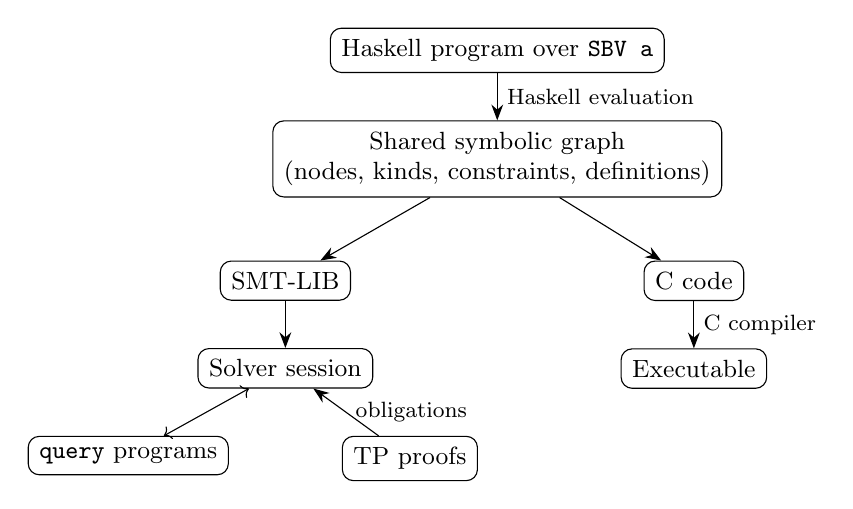
\begin{tikzpicture}[node distance=6mm and 8mm,
    box/.style={draw,rounded corners,align=center,inner sep=4pt,font=\small},
    arr/.style={-{Stealth[length=2mm]}}]
\node[box] (hs) {Haskell program over \code{SBV a}};
\node[box,below=of hs] (graph) {Shared symbolic graph\\(nodes, kinds, constraints, definitions)};
\node[box,below left=8mm and -10mm of graph] (smt) {SMT-LIB};
\node[box,below right=8mm and -10mm of graph] (c) {C code};
\node[box,below=of smt] (solver) {Solver session};
\node[box,below left=6mm and -4mm of solver] (q) {\code{query} programs};
\node[box,below right=6mm and -4mm of solver] (tp) {TP proofs};
\node[box,below=of c] (exe) {Executable};
\draw[arr] (hs) -- node[right,font=\footnotesize]{Haskell evaluation} (graph);
\draw[arr] (graph) -- (smt);
\draw[arr] (graph) -- (c);
\draw[arr] (smt) -- (solver);
\draw[arr] (c) -- node[right,font=\footnotesize]{C compiler} (exe);
\draw[arr,<->] (q) -- (solver);
\draw[arr] (tp) -- node[right,font=\footnotesize]{obligations} (solver);
\end{tikzpicture}
\caption{Haskell evaluation builds a shared graph, which is translated to SMT-LIB
for the solver or to C for execution. Queries and proofs drive the solver.}
\Description{A Haskell program over symbolic values is evaluated into a shared
symbolic graph. The graph is translated either to SMT-LIB, feeding a solver
session that query programs and TP proofs interact with, or to C code.}
\label{fig:architecture}
\end{figure}

\paragraph{Symbolic values are deferred graph nodes.}
Internally, a value of type \code{SBV a} is either a concrete constant or a
deferred computation that, given the state of the current symbolic run, adds a
node to a graph and returns its identifier:
\begin{lstlisting}
newtype SBV a = SBV SVal
data SVal     = SVal Kind (Either CV (Cached SV))
newtype Cached a = Cached (State -> IO a)
\end{lstlisting}
This representation lets \code{\textbackslash{}x y -> x + y} have the pure type
\code{SWord8 -> SWord8 -> SWord8} while still allocating graph nodes. Operations
on constants are folded immediately, which is why \code{satAdd 250 10} evaluates
to \code{255} without a solver. The run-time \code{Kind} records the logical sort,
so simplifications can respect it: rewriting \code{x .== x} to true is valid for
integers but not for floats.

\paragraph{Sharing comes in two forms.}
A generator that combines a term with itself, such as
\code{iterate (\textbackslash{}t -> t + t) x !! 30}, describes a term that is
exponentially large as a tree but linear as a graph. SBV preserves this sharing
in two ways. It memoizes each deferred computation, using stable names in the
style of observable sharing~\citep{sharing}, so that forcing the same Haskell
value twice yields the same node. It also interns nodes, so that separately
constructed applications of the same operator to the same arguments reuse a node.
Neither mechanism identifies arbitrary mathematically equal expressions.

\paragraph{Nodes belong to a run.}
A graph node is meaningful only in the run that created it. Two values of type
\code{SInteger} from different calls to \code{prove} cannot be combined, even
though their types agree, and SBV checks for common mistakes of this kind. To
carry a result from one run to another, extract a concrete value from a model
and turn it back into a literal. Section~\ref{sec:queries} illustrates the same
concrete-to-symbolic conversion with \code{literal v}, though its loop stays
within one run. Constants and reusable function definitions can be shared
across runs; session-specific symbolic unknowns cannot.

\paragraph{Queries synchronize dependencies.}
When a query creates a new term, SBV records the declarations it requires: sorts
for datatypes (including those nested inside lists, tuples, or other datatypes),
uninterpreted constants, and definitions of \code{smtFunction}s it calls. Before
the term is used, any of these that the solver has not seen are sent. This is why
a datatype can first appear inside a query. The companion exercises this case
with two fresh values of a parameterized datatype created by \code{freshVar}.

\subsection{Termination is a proof obligation}
\label{sec:termination}

The \code{Functions proven terminating} line in TP output records a check that
is separate from the theorem's induction. SMT functions denote total functions.
An arbitrary recursive equation need not define one: for example,
$b(n)=b(n)+1$ has no integer-valued solution. Admitting that equation as a
definition would make the logical context inconsistent, allowing unrelated
claims to be proved. Haskell's willingness to accept a recursive definition is
therefore insufficient for using it in a proof.

When SBV registers a recursive \code{smtFunction}, it records a deferred
termination check along with the definition. Automatic checks try measures
suggested by the argument types, such as list length or datatype size. For a
measure $m$ and each recursive call from arguments $\vec{x}$ to $\vec{x}'$,
the obligations have the form
\[
 m(\vec{x})\geq 0,
 \qquad C(\vec{x})\Longrightarrow m(\vec{x}')<m(\vec{x}),
\]
where $C$ is the condition under which that call is reached. The ordering must
be well founded: nonnegative integers cannot decrease forever. For
\code{sumL}, a recursive call is reached only in the nonempty-list branch,
where the tail is one element shorter. Checking a proper datatype subterm can
also be done structurally, without a solver query. Mutual recursion is checked
across calls between members of the recursive group, not just self-calls.

TP gathers these checks from the definitions encountered while constructing a
lemma or calculation, including functions used by its dependencies. Before
checking the proof, it verifies newly encountered measures and remembers the
successful checks within that TP run. At the end, \code{runTP} audits that no
encountered check was left outstanding and reports the verified functions.
This is why \code{sumNonNeg} reports both \code{sumL} and the library fold
used to express its premise. These checks concern the symbolic definitions
actually encountered, not every Haskell function in the source module.

If an automatic measure cannot be established, SBV rejects the definition and
requests an explicit one via \code{smtFunctionWithMeasure}; an unknown solver
answer does not establish termination. The normalizer in
Section~\ref{sec:tautology} illustrates a lexicographic measure and proved helper
lemmas. The companion also checks that a definition with the equation
$b(n)=b(n)+1$ is rejected. Explicitly choosing
\code{smtFunctionNoTermination} bypasses the check, but TP records that
assumption in the proof's dependencies and reports the result as
\code{Modulo} the function's termination. Such a result is conditional, not
evidence that the function terminates. Productivity checks for corecursive
definitions are a separate facility, outside this tutorial's finite-list setting.

\subsection{Why finite lists and datatypes?}
\label{sec:finite-lists}

SBV's \code{SList a} denotes finite SMT sequences, excluding Haskell's bottom,
$\bot$, in both spine and elements. Thus \code{[undefined]},
\code{1 : undefined}, and \code{repeat 0} are outside the model. Every
symbolic-list proof has this restriction, including at all levels of nested
lists. ``Arbitrary length'' means no finite bound is imposed; infinity is not
another possible length.

Finiteness is not specific to lists. SBV supports algebraic datatypes with
recursive fields, but their SMT interpretations likewise contain only finite,
total constructor trees, including with mutual or nested recursion.
\code{SExpr} from Section~\ref{sec:datatypes} admits finite trees of arbitrary
size; the cyclic Haskell value \code{e = Add (Num 1) e} has no counterpart.
All fields must be defined and recursive structure must terminate. Datatype
proofs therefore have the same finite, total scope as list proofs.
This restriction concerns recursive constructor structure. Arrays instead use
the total-mapping semantics of Section~\ref{sec:arrays}, with potentially
infinite index domains.

The distinction matters even for familiar equations. Reversing twice is the
identity on finite lists, but consider the ordinary Haskell value
\code{xs = repeat 0}. The expression \code{take 1 xs} produces \code{[0]},
whereas \code{take 1 (reverse (reverse xs))} diverges: the first reversal never
reaches the end. A finite-list theorem therefore cannot justify this rewrite
for an arbitrary lazy Haskell list. Likewise, a termination argument based on
decreasing length presupposes a finite length; it does not establish productivity
on infinite input.

We choose this boundary because it aligns reasoning with the solver's finite
sequences and inductive datatypes, giving TP a direct structural induction principle and a
natural termination measure. It covers the folds, accumulator algorithms, and
transformations of finite data developed here. Extending the domain would require
additional semantics and proof rules: reasoning about partial approximations
must account for definedness and strictness, while infinite streams require a
suitable representation and coinductive reasoning. Merely adding a bottom case
to list induction cannot create infinite values in the SMT sequence sort.
Keeping these concerns outside the sequence and inductive datatype models limits
the machinery whose soundness these proofs depend on.

This choice is consistent with the motivation of
\citet{fastloose}. For their specified languages, equality proved in a total
semantics yields a relation between values in a partial semantics. For their
example on lists of natural numbers, this recovers equality on total, finite
inputs; at function types,
the relation compares behavior on related inputs. Their result explains how
total reasoning can avoid repeatedly propagating definedness conditions. It is
not a transfer theorem for SBV or all of Haskell: applying an SBV result to a
Haskell implementation still requires matching its operations and input domain
to the symbolic model.

When a problem concerns streams, a separate model may suffice. For example,
representing a stream by an index function $s : \mathbb{N}\to A$ turns equality
into pointwise equality and suits uniform operations such as map and zip.
That is a different specification, not an extension of a theorem over
\code{SList}; operations such as filtering require further reasoning.

%==============================================================================
\section{Pitfalls and What to Trust}
\label{sec:pitfalls}

\paragraph{Common pitfalls.}
\begin{itemize}
\item \emph{Wrong domain.} A property proved over \code{SInteger} says nothing
  about \code{SInt32}, and vice versa. Choose the type that matches the code you
  care about. List and recursive-datatype theorems cover finite, total values only
  (Section~\ref{sec:finite-lists}).
\item \emph{Specification repeats the implementation.} Write specifications in a
  different style or a wider domain (Section~\ref{sec:specs}).
\item \emph{Haskell \code{if} or recursion on symbolic data.} Use \code{ite} and
  \code{sCase} for symbolic choices, and \code{smtFunction} for recursion over
  symbolic structure (Section~\ref{sec:host}).
\item \emph{Contradictory assumptions.} If \code{constrain}ed assumptions are
  unsatisfiable, everything is provable. A quick \code{sat} on the assumptions
  alone detects this.
\item \emph{Treating unknown as an answer.} A timeout or unknown result is
  neither a proof nor a counterexample.
\item \emph{Too specific an induction statement.} If a proof step involving the
  induction hypothesis fails, the statement probably needs generalizing
  (Sections~\ref{sec:induction} and~\ref{sec:kadane}).
\item \emph{Mixing runs.} Unknowns belong to the run that created
them; move concrete values instead (Section~\ref{sec:hood}).
\end{itemize}

\paragraph{What a proof rests on.}
A Q.E.D. from SBV depends on the correctness of SBV's translation to SMT-LIB, the
solver, and, for TP, the generation of proof obligations. TP proofs also depend on
any axioms the user introduces and on any functions whose termination checks
were explicitly bypassed. SBV tracks these dependencies: a proof that rests on an
axiom, or on an unfinished step marked with \code{sorry}, is reported as
\code{Modulo} the offending lemmas rather than as \code{Proven}. TP does not replay solver certificates in an independent proof
kernel, so its guarantees are those of the underlying solver. For generated C, the C compiler
and the code generator join the trusted base, which is why
Section~\ref{sec:codegen} validates the generated code separately.

%==============================================================================
\section{Related Tools and Further Reading}
\label{sec:related}

QuickCheck~\citep{quickcheck} and SBV ask similar questions with different
evidence: a passing test campaign samples the input space, while an
unsatisfiability result covers it. The two combine well, and SBV's own test
suite compares concrete evaluation with solver results using QuickCheck.

Several systems embed solver-aided programming in a host language.
Rosette~\citep{rosette} provides a symbolic virtual machine for Racket that
lifts ordinary host constructs to symbolic values. Grisette~\citep{grisette} is
a Haskell library for symbolic compilation that focuses on efficient symbolic
evaluation of programs with state merging. Smten~\citep{smten} translated
high-level Haskell-like symbolic computations into SMT queries. The what4
library~\citep{what4} offers a typed Haskell interface to many solvers and is
used inside verification tools. SBV makes the boundary between Haskell and
symbolic control explicit through its types and operators, and adds the TP proof
layer and C generation on the same representation.

For proofs about Haskell programs, Liquid Haskell~\citep{liquidhaskell} checks
refinement types with an SMT solver, and refinement reflection~\citep{reflection}
extends it to equational proofs about user-defined functions. There, specifications
are refinement types on the program itself and proofs are Haskell terms checked
against them; SBV's TP proofs are instead separate Haskell programs about
symbolic models. Dafny~\citep{dafny} shows
how far the combination of user-supplied invariants and automatic
verification-condition discharge can go in a dedicated language.

The SBV distribution contains a large collection of documented examples under
\code{Documentation.\allowbreak SBV.\allowbreak Examples}, covering puzzles, cryptography, code
generation, optimization, and theorem proving. The TP examples mentioned in
Section~\ref{sec:tautology} are a good next step after this tutorial.

%==============================================================================
\section{Conclusion}

SBV connects constraint solving, optimization, and inductive proofs through one
vocabulary of symbolic values. Effective use depends on choosing the right
semantic domain, writing independent specifications, separating Haskell from
symbolic control, and generalizing induction hypotheses. The companion provides
executable models and checked calculations that readers can adapt to their own
programs.

\bibliographystyle{ACM-Reference-Format}
\bibliography{references}
\end{document}
